% CS301 Computer Networks -- Mini-Project Progress Report
% Layout cloned from the CS255 FEC report (Sem IV).
\documentclass[11pt,a4paper]{article}

% ---------------------------------------------------------------- report metadata
\newcommand{\CourseLine}{CS301 --- Computer Networks}
\newcommand{\ReportLine}{Mini-Project Progress Report}
\newcommand{\HeaderLeft}{CS301 Mini-Project Progress Report}
\newcommand{\HeaderRight}{Team T7 \textbar{} 241CS222, 241CS243, 241CS257}
\newcommand{\RepoName}{somyaknotfound/S2-T7}
\newcommand{\RepoURL}{https://github.com/somyaknotfound/S2-T7}

% ---------------------------------------------------------------- packages
\usepackage[utf8]{inputenc}
\usepackage[T1]{fontenc}
\usepackage[margin=1in]{geometry}
\usepackage{setspace}
\usepackage{amsmath,amssymb}
\usepackage{graphicx}
\usepackage{booktabs}
\usepackage{array}
\usepackage{tabularx}
\usepackage[table]{xcolor}
\usepackage{enumitem}
\usepackage{titlesec}
\usepackage{fancyhdr}
\usepackage{caption}
\usepackage{float}
\usepackage{algorithm}
\usepackage{algpseudocode}
\usepackage{tikz}
\usetikzlibrary{positioning,arrows.meta,shapes.geometric}
\usepackage{hyperref}

\hypersetup{
  colorlinks=true,
  linkcolor=blue!70!black,
  citecolor=blue!70!black,
  urlcolor=blue!80!black,
  pdftitle={\HeaderLeft},
}

% ---------------------------------------------------------------- spacing
\setstretch{1.1}
\setlength{\parindent}{0pt}
\setlength{\parskip}{4pt}
\renewcommand{\arraystretch}{1.45}
\setlength{\intextsep}{8pt plus 2pt minus 2pt}

% ---------------------------------------------------------------- headings: "1. Title" with rule, "1.1. Title"
\titleformat{\section}{\Large\bfseries}{\thesection.}{0.5em}{}[\vspace{-0.5ex}\titlerule]
\titleformat{\subsection}{\large\bfseries}{\thesubsection.}{0.5em}{}
\titleformat{\subsubsection}{\normalsize\itshape}{\thesubsubsection.}{0.5em}{}
\titlespacing*{\section}{0pt}{3ex plus 1ex}{1.5ex}
\titlespacing*{\subsection}{0pt}{2.5ex plus 1ex}{1ex}
\titlespacing*{\subsubsection}{0pt}{2ex plus 1ex}{0.8ex}

% ---------------------------------------------------------------- header / footer
\pagestyle{fancy}
\fancyhf{}
\fancyhead[L]{\HeaderLeft}
\fancyhead[R]{\HeaderRight}
\fancyfoot[C]{\thepage}
\renewcommand{\headrulewidth}{0.4pt}
\setlength{\headheight}{14pt}

% ---------------------------------------------------------------- captions, lists
\captionsetup{font=normalsize, labelsep=colon, skip=6pt}
\captionsetup[table]{position=top}
\setlist[enumerate]{leftmargin=*, itemsep=2pt}
\setlist[itemize]{leftmargin=*, itemsep=2pt}

% ---------------------------------------------------------------- house macros
\newcommand{\pros}{\textcolor{green!50!black}{\textbf{Pros:}}~}
\newcommand{\cons}{\textcolor{red!70!black}{\textbf{Cons:}}~}
\newcommand{\code}[1]{\texttt{#1}}
\newcommand{\Dup}{\widehat{D}_{\mathrm{up}}}

% pastel boxes used in every TikZ figure
\tikzset{
  box/.style={draw=black!60, rounded corners=2pt, align=center, inner sep=4pt, minimum height=1.0cm},
  orangebox/.style={box, fill=orange!10},
  greenbox/.style={box, fill=green!10},
  bluebox/.style={box, fill=blue!8},
  graybox/.style={box, fill=black!5},
  arr/.style={-{Stealth[length=2mm]}, thick},
}

\begin{document}

% ================================================================ TITLE PAGE
\hypersetup{pageanchor=false}
\begin{titlepage}
\centering
\vspace*{0.6cm}
{\large\bfseries National Institute of Technology Karnataka, Surathkal\par}
\vspace{6pt}
{\large\bfseries Department of Computer Science and Engineering\par}
\vspace{18pt}
{\CourseLine\par}
\vspace{6pt}
{\ReportLine\par}
\vspace{1.4cm}

\rule{\linewidth}{1pt}\par
\vspace{0.35cm}
{\LARGE\bfseries\setstretch{1.55}
Threshold-Aware Similarity Caching\\
for Named Data Networks:\\
Bounding Retry Delay\\
under Congestion using ns-3\par}
\vspace{0.25cm}
\rule{\linewidth}{1pt}\par

\vspace{1.0cm}
{\bfseries Project Repository\par}
\vspace{6pt}
\href{\RepoURL}{\small\texttt{\RepoName}}\par

\vspace{1.0cm}
\begin{tabular}{@{}r@{\hspace{8pt}}l@{}}
  \textbf{Students:} & Somyak Priyadarshi Mohanta (241CS257) \\[-4pt]
                     & Pranav Shaji (241CS243) \\[-4pt]
                     & Chris Tony (241CS222) \\[4pt]
  \textbf{Department:} & Computer Science and Engineering \\[-4pt]
  \textbf{Institute:}  & National Institute of Technology Karnataka, Surathkal \\
\end{tabular}

\vspace{0.8cm}
\begin{tabular}{@{}r@{\hspace{8pt}}l@{}}
  \textbf{Guide:}      & Prof. B. R. Chandavarkar \\[-4pt]
  \textbf{Department:} & Computer Science and Engineering, NITK \\
\end{tabular}
\vfill
\end{titlepage}
\hypersetup{pageanchor=true}

% ================================================================ ABSTRACT
\setcounter{page}{1}
\begin{abstract}
Routers in Named Data Networking (NDN) may keep a copy of every Data packet they forward, yet a
conventional cache replies only when it holds the very object an Interest names~\cite{zhang2014ndn}.
Similarity caching loosens that rule: on a miss, the cache may hand back the stored object that
comes closest to the request. Image retrieval, recommendation engines and the semantic caching of
large language-model queries all gain from this~\cite{neglia2022similarity,schroeder2025vcache}.
The client, however, still judges whether the reply is close enough, and asks again when it is not.

Those repeat requests are hard to control once a request crosses several caches. A cache rarely
knows how much similarity a given client will tolerate, and NDN's name matching limits how a
substitute can be sent back. Worse, the contents of a cache barely change between two retries a few
milliseconds apart, so a client can be handed the same unsuitable answer again and again. Forwarding
is not free either: its cost grows with queueing and loss on the upstream path. Nakamura and
Kamiyama~\cite{nakamura2024analysis} analyse delivery delay in cache networks, but they assume one
fixed answer probability $\alpha$, perfect links, and retries that behave as if the cache contents
were drawn afresh each time.

In this project we build threshold-aware similarity caching for NDN and evaluate it in ns-3 with
ndnSIM~\cite{mastorakis2017ndnsim}. An Interest can either state the lowest similarity the client
will accept or list the caches whose earlier answers were turned down. On top of this, we study a
delay-aware rule that weighs the expected cost of answering locally against the measured cost of
sending the request upstream. Our three objectives are to reproduce the base paper at packet level
and study what persistent cache contents do to delay; to design threshold and exclusion signalling
that caps the number of retries and admits a closed-form delay; and to compare a congestion- and
loss-aware rule with fixed-$\alpha$ caching. So far, the simulator agrees with the analytical model
in all 18 configurations of the base paper's setting. When contents persist and $\alpha=0.9$, the
mean delay climbs from 80.6~ms to 14.5~s. Carrying the threshold in the Interest removes this long
tail in our tests: the mean drops to 4.84~ms, with a single attempt. Under backhaul congestion and
burst loss, the delay-aware rule beats the best fixed $\alpha$ at every operating point we tried, by
2.8 to 20.8~ms.
\end{abstract}

\vspace{1em}
\noindent\textbf{Keywords:} Similarity caching, Named Data Networking, Information-Centric
Networking, retry delay, congestion, burst loss, ns-3, ndnSIM.

\newpage
% ================================================================ CONTENTS
{\setlength{\parskip}{0pt}\setstretch{1.15}\tableofcontents}
\newpage

% ================================================================ 1 INTRODUCTION
\section{Introduction}\label{sec:intro}

\subsection{Background}
Caching places copies of popular objects near the people who ask for them, so a request travels
fewer hops, is answered sooner and puts less load on upstream links. Information-Centric Networking
goes a step further and makes caching a job of the network itself, not just of application servers.
In Content-Centric Networking~\cite{jacobson2009ccn} and its successor, Named Data Networking
(NDN)~\cite{zhang2014ndn}, a consumer issues an Interest packet that names the data it needs. Any
router on the way can reply from its Content Store; the Data packet then retraces the Interest's
path, and each router it passes may keep a copy.

Almost every NDN caching and placement scheme obeys one strict rule: a router replies only if it
holds exactly the object the Interest names~\cite{chaudhary2026ndncaching}. Similarity caching
relaxes this. If the exact object is missing, the cache may return its closest match, giving up a
little accuracy for a possibly much shorter path. The idea goes back to metric caches for
content-based image search~\cite{falchi2008metric} and to nearest-neighbour caches for contextual
advertising~\cite{pandey2009nn}. It has since been treated as a general caching problem, with uses in
multimedia retrieval, recommender systems and machine-learning services~\cite{neglia2022similarity}.
Its most visible use today is the semantic caching of large language-model (LLM) queries, where a
stored answer to a prompt with the same meaning can spare an expensive
inference~\cite{bang2023gptcache,gill2025meancache,schroeder2025vcache}.

In each of these settings the client, or the application acting for it, checks whether the reply is
good enough and asks again if it is not. What matters to the user, then, is not how often a single
cache hits, but how long it takes for an acceptable answer to arrive.

\subsection{Challenges and Issues}
Spreading similarity caching over a multi-hop network brings four difficulties. The first is that a
cache usually does not know the lowest similarity a given user will accept. Under a blind rule, such
as the one Nakamura and Kamiyama~\cite{nakamura2024analysis} analyse, a cache may send back an answer
that is bound to be rejected. That reply still costs a full round trip, plus the retry interval
$\delta$ before the next attempt.

The second is that cache contents hardly change in the short gap between retries. If the caches near
a user hold nothing above the user's threshold, the retry meets the same unsuitable objects and gets
the same rejected answers. The attempts are therefore correlated, not independent. In the base
paper's own setting, we find that this persistence raises the mean delay by up to 2.1 times at
$\alpha=0.5$ and by roughly 1700 times at $\alpha=0.9$, relative to what the model predicts.

The third comes from the protocol. NDN delivers Data only when its name matches a pending
Interest~\cite{zhang2014ndn}, so a cache cannot send a substitute under the substitute's own name
while the forwarders are waiting for the original one. We keep the Interest--Data name match as it is
and place the identity and similarity of the served object in the payload.

The fourth is that the worth of a nearby approximate answer depends on what lies upstream. When the
backhaul is congested or drops packets in bursts~\cite{gilbert1960capacity,elliott1963estimates},
forwarding is slow and a local reply is worth more. When the upstream path is quiet, forwarding is
cheap and an approximate reply is seldom worth the risk of rejection. A cache therefore needs a
running estimate of its forwarding delay, much as TCP keeps one for its retransmission
timer~\cite{jacobson1988congestion,paxson2011rfc6298}. None of these effects shows up without
packet-level simulation, which calls for an NDN simulator extended with a similarity-aware Content
Store and a matching forwarding strategy~\cite{mastorakis2017ndnsim}.

\subsection{Existing Approaches and Their Issues}
Most of the similarity-caching literature looks at a single cache and asks what it should hold and
how often it can serve a request. This line of work includes metric caches for
search~\cite{falchi2008metric}, nearest-neighbour caching~\cite{pandey2009nn}, the theory and dynamic
policies of Neglia et al.~\cite{neglia2022similarity}, online caching with approximate
indexes~\cite{sisalem2023acai}, hit-rate analysis through time-to-live (TTL)
approximations~\cite{benmazziane2024ttl}, and learned per-prompt thresholds for LLM
caches~\cite{schroeder2025vcache}. At the network level, studies decide where to place content across
several similarity caches~\cite{garetto2021placement} or learn cooperative policies for edge
nodes~\cite{wang2025bandit}.

All of these tune a cost or a caching policy, but none models a user who turns down an answer and
tries again. Nakamura and Kamiyama~\cite{nakamura2024analysis} do model the delay a user sees over a
path of caches, yet they assume a single answer probability $\alpha$, ideal links with unlimited
bandwidth and independent retries, and they evaluate the model only numerically. What remains open
is how each cache should choose between an approximate local reply and forwarding the Interest,
given the user's tolerance and the present state of the upstream path. None of the works above
examines that choice with packet-level NDN simulation.

\subsection{Problem Statement}
Consider an NDN network of similarity caches whose users accept an answer only if its similarity
meets their own threshold, and whose upstream links may be congested or lossy. The goal is to design
the request signalling and a per-cache answer-or-forward rule that keep retries bounded and cut the
mean delay until an acceptable answer arrives. Where the analysis allows, the delay is derived in
closed form, and the design is validated at packet level in ns-3 with ndnSIM.

\subsection{Objectives}
\begin{enumerate}[label=\textbf{O\arabic*.}]
  \item Build similarity caching with client retries in ns-3/ndnSIM, reproduce the base paper's
        delay model on its tandem topology, and measure how the delay changes when cache contents
        persist between retries.
  \item Design threshold-carrying and exclusion Interests that put an upper bound on retries, and
        derive the resulting delay in closed form.
  \item Develop a delay-aware answer-or-forward rule that learns user acceptance and upstream delay
        while it runs, and compare it with fixed-$\alpha$ caching under backhaul congestion and burst
        loss in terms of mean and tail delay, delivered similarity and upstream traffic.
\end{enumerate}

\subsection{Organisation of the Report}
The remainder of the report is arranged as follows. Section~\ref{sec:lit} surveys earlier work in
the order it appeared and contrasts the approaches in Section~\ref{sec:lit-compare}.
Section~\ref{sec:approach} sets out our approach: the system model (Section~\ref{sec:system}), the
answer-or-forward policies (Section~\ref{sec:policies}), the delay-aware algorithm
(Section~\ref{sec:algo}) and the reasons behind these design choices (Section~\ref{sec:justify}).

% ================================================================ 2 LITERATURE REVIEW
\section{Literature Review}\label{sec:lit}

This section reviews eight approaches in chronological order (Fig.~\ref{fig:timeline}), from the
first single-cache systems to recent semantic and cooperative caching, and ends with a comparison
that pins down the gap we target.

\begin{figure}[H]
\centering
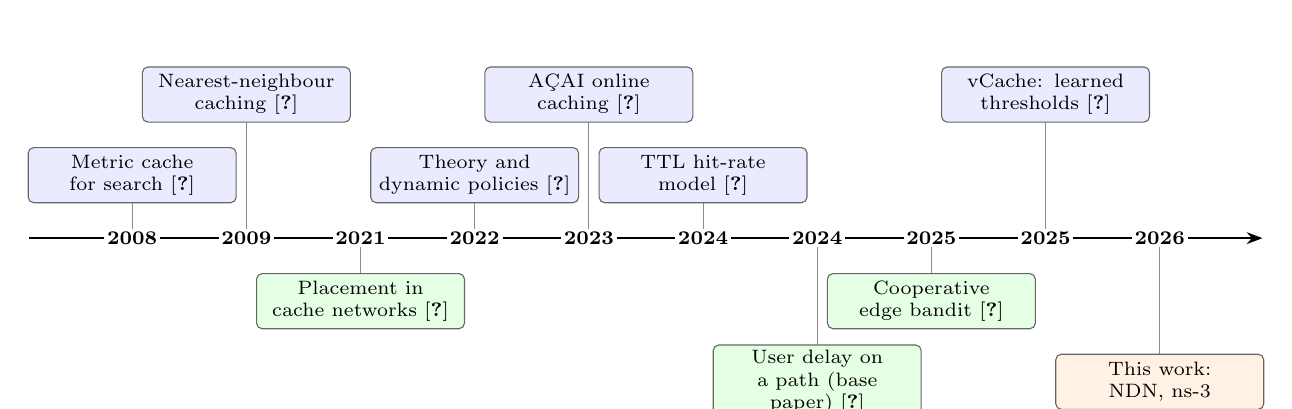
\begin{tikzpicture}[x=1.45cm, y=0.64cm,
    ev/.style={font=\scriptsize, text width=2.5cm, minimum height=0.7cm, inner sep=2pt,
               execute at begin node={\hyphenpenalty=10000\exhyphenpenalty=10000}},
    yr/.style={font=\scriptsize\bfseries, fill=white, inner sep=1pt}]
  \draw[thick, -{Stealth[length=2mm]}] (-0.9,0) -- (9.9,0);
  \def\event#1#2#3#4#5{%
    \draw[black!45] (#1,0) -- (#1,#2);
    \node[#4, ev] at (#1,#2) {#5};
    \node[yr] at (#1,0) {#3};}
  \event{0}{1.25}{2008}{bluebox}{Metric cache for search~\cite{falchi2008metric}}
  \event{1}{2.85}{2009}{bluebox}{Nearest-neighbour caching~\cite{pandey2009nn}}
  \event{2}{-1.25}{2021}{greenbox}{Placement in cache networks~\cite{garetto2021placement}}
  \event{3}{1.25}{2022}{bluebox}{Theory and dynamic policies~\cite{neglia2022similarity}}
  \event{4}{2.85}{2023}{bluebox}{A\c{C}AI online caching~\cite{sisalem2023acai}}
  \event{5}{1.25}{2024}{bluebox}{TTL hit-rate model~\cite{benmazziane2024ttl}}
  \event{6}{-2.85}{2024}{greenbox}{User delay on a path (base paper)~\cite{nakamura2024analysis}}
  \event{7}{-1.25}{2025}{greenbox}{Cooperative edge bandit~\cite{wang2025bandit}}
  \event{8}{2.85}{2025}{bluebox}{vCache: learned thresholds~\cite{schroeder2025vcache}}
  \event{9}{-2.85}{2026}{orangebox}{This work: NDN, ns-3}
\end{tikzpicture}
\caption{Reviewed approaches by year (not to scale): one cache above the axis, a network below.}
\label{fig:timeline}
\end{figure}

\subsection{Early Similarity Caches (Falchi et al., 2008; Pandey et al., 2009)}
Falchi et al.~\cite{falchi2008metric} put a cache in front of a content-based image search engine, so
that a new query could reuse the stored results of an earlier, similar nearest-neighbour query.
Pandey et al.~\cite{pandey2009nn} carried the same idea over to contextual advertising: a request is
served if a similar page is already in the cache. They examined caching policies under two
efficiency--accuracy goals and bounded the achievable gain under a generative model of page requests.

\pros They were the first to show that similar requests can share cached results, easing the load on
the back end.\\
\cons Both use a single cache in front of one server and a fixed answer rule, and neither accounts
for network delay.

\subsection{Placement in Networks of Similarity Caches (Garetto et al., 2021)}
Garetto, Leonardi and Neglia~\cite{garetto2021placement} moved the problem into networks. A request
travels along a path of similarity caches, and objects are placed so that the path as a whole strikes
a good balance between efficiency and accuracy. Placing objects offline is NP-hard, though
polynomial-time algorithms come close to the optimum in discrete cases, and a continuous version of
the problem has a simple optimal structure on trees.

\pros A network-wide view of similarity caching, backed by structural results.\\
\cons Placement is computed offline with a fixed cost per hop; queueing, loss, retries and protocol
behaviour are left out.

\subsection{Similarity Caching: Theory and Algorithms (Neglia et al., 2022)}
Neglia, Garetto and Leonardi~\cite{neglia2022similarity} analyse one similarity cache in the offline,
adversarial and stochastic settings. Serving a similar object costs some utility, more the less
similar it is, while a miss costs a retrieval fee. They also give the first dynamic policies with
optimality guarantees.

\pros A rigorous cost model and dynamic policies with provable guarantees.\\
\cons Only one cache is studied; the retrieval cost is not a measured network delay, and users never
reject an answer or retry.

\subsection{Ascent Similarity Caching with Approximate Indexes (Si Salem et al., 2023)}
Si Salem, Neglia and Carra~\cite{sisalem2023acai} propose A\c{C}AI for edge servers. An approximate
index over the whole catalogue tells the server whether to answer a request locally or fetch it from
a remote server, and mirror ascent updates the cached set. Its guarantees hold even when requests
follow no statistical pattern.

\pros Guarantees under adversarial requests, built on practical approximate indexes.\\
\cons One edge cache only; congestion and loss on the path to the remote server are not modelled.

\subsection{TTL Model for an LRU-Based Similarity Cache (Ben Mazziane et al., 2024)}
Ben Mazziane et al.~\cite{benmazziane2024ttl} carry the time-to-live (TTL) approximation of classical
caching over to an LRU-based similarity caching policy. A TTL cache, tuned through a fixed-point
system of equations to mimic the policy, yields its hit rate without any simulation.

\pros A tractable way to obtain hit rates, which could feed models of cache contents.\\
\cons It covers one cache and its hit rate only; neither end-to-end delay nor a network is modelled.

\subsection{Similarity Caching on Cache Networks (Nakamura and Kamiyama, 2024)}
In our base paper~\cite{nakamura2024analysis}, a request follows a fixed path of caches towards the
origin. On a miss, each cache replies with its most similar object with probability $\alpha$ and
otherwise passes the Interest on. The client accepts a reply only if its similarity is at least $s$;
if not, it waits $\delta$ and tries again. Writing $\rho$ for the probability that an attempt is
accepted, and $d_{\geq}$ and $d_{<}$ for the mean delays of accepted and rejected attempts, the paper
gives the mean delivery delay as
\begin{equation}
  \mathbb{E}[D] = d_{\geq} + \left(\frac{1}{\rho}-1\right)(d_{<}+\delta),
  \label{eq:base-delay}
\end{equation}
and evaluates it numerically on a tandem of five caches.

Re-deriving the model revealed three issues. The path delay printed as Equation~(6) of the base paper uses only the last-hop round trip, while its figures
appear to use the cumulative one. With that corrected, our values match Fig.~5(a) of the paper at
$s=1$ for $\alpha=0.1$ and $0.5$ (9.96~ms and 45.97~ms) and come close at $\alpha=0.9$ (80.6~ms).
Equations~(8) and~(10) of the paper also seem to rest on different assumptions: one describes a
cache that knows $s$, the other a cache that is blind to it. Most importantly,
Eq.~\eqref{eq:base-delay} averages $\rho$ as if every retry redrew the cache contents independently.
When the contents persist, Jensen's inequality gives $\mathbb{E}[1/\rho] \geq 1/\mathbb{E}[\rho]$ for
the expected number of attempts, so the model can underestimate the delay.

\pros The first closed-form, user-level delay metric for retries over a path of caches.\\
\cons One global $\alpha$, applied even to exact hits; ideal links; independent retries; and a purely
numerical evaluation with no packet-level simulation.

\subsection{Similarity Caching in Cooperative Edge Networks (Wang et al., 2025)}
Wang et al.~\cite{wang2025bandit} consider edge nodes that cooperate to serve requests over links
whose quality varies. They cast caching as an adversarial multi-armed bandit and propose MABSCP, an
online policy that adjusts the cached sets from feedback to trade similarity against delivery
latency.

\pros Online and cooperative; latency enters the cost, and the policy adapts as conditions change.\\
\cons It chooses what to cache, not whether to answer a given request; latency is not measured on the
network, and retries are not modelled.

\subsection{Verified Semantic Prompt Caching (Schroeder et al., 2025)}
vCache~\cite{schroeder2025vcache} reuses a stored LLM response when a new prompt's embedding lies
close to that of a cached prompt. Instead of one fixed similarity threshold, it learns a separate
threshold for every cached prompt, so that the cache stays within an error rate chosen by the user.

\pros It answers only when acceptance is likely, learned from feedback, which makes it the closest in
spirit to our rule.\\
\cons It is a single server-side cache that targets answer correctness, not network delay, and has no
multi-hop path.

\subsection{Comparison of Existing Approaches}\label{sec:lit-compare}
Table~\ref{tab:related-work} sets the reviewed approaches side by side.

\begin{table}[H]
\centering
\caption{Comparison of similarity-caching approaches}
\label{tab:related-work}
\footnotesize
\renewcommand{\arraystretch}{1.0}
\begin{tabularx}{\linewidth}{@{}>{\raggedright}p{3.2cm}>{\raggedright}p{1.8cm}>{\raggedright}X>{\raggedright}p{2.7cm}>{\raggedright\arraybackslash}p{2.4cm}@{}}
\toprule
\textbf{Approach} & \textbf{Scope} & \textbf{Main decision} & \textbf{Rejections / retries} &
\textbf{Upstream delay / loss} \\
\midrule
Falchi~\cite{falchi2008metric}, Pandey~\cite{pandey2009nn} & One cache & What to store & No & No \\
Garetto~\cite{garetto2021placement} & Path / tree & Offline placement & No & No \\
Neglia~\cite{neglia2022similarity} & One cache & What to store & No & No \\
Si Salem~\cite{sisalem2023acai} & One cache & What to store, online & No & No \\
Ben Mazziane~\cite{benmazziane2024ttl} & One cache & Hit-rate analysis & No & No \\
Nakamura~\cite{nakamura2024analysis} & Path & Answer with fixed $\alpha$ & Independent retries & No \\
Wang~\cite{wang2025bandit} & Edge nodes & What to store, online & No & Latency is a cost \\
Schroeder~\cite{schroeder2025vcache} & One cache & Learned answer threshold & No & No \\
\midrule
\textbf{This work} & \textbf{NDN path} & \textbf{Per-request answer or forward} &
\textbf{Correlated; bounded by signalling} & \textbf{Measured online} \\
\bottomrule
\end{tabularx}
\end{table}

The gap lies in the decision each cache takes. Single-cache work settles what to store but never
sees the network path; placement studies span several caches but ignore users who reject and retry;
and the base paper models retries, but with blind caches, independent attempts and an ideal network.
We ask whether a cache can decide, request by request, from the similarity it can offer and its own
estimate of upstream delay, and we test that decision at packet level in an NDN simulator.

% ================================================================ 3 PROPOSED APPROACH
\section{Proposed Approach}\label{sec:approach}

\subsection{System Model}\label{sec:system}
We keep the base paper's tandem topology, so our results can be set directly against its model, and
add congestion and burst loss on top (Fig.~\ref{fig:system}). Five caches and an origin are joined by
1~Gbps links with a 1~ms delay, and client $c_i$ sits at cache $v_i$. The catalogue holds $C=100$
items, each cache stores $B=10$ of them, and a client whose answer is rejected waits $\delta=10$~ms
before trying again.

In the congestion runs, the link from $v_5$ to the origin becomes a 2~Mbps backhaul with a 100-packet
DropTail queue, which it shares with Poisson cross traffic from $v_1$. In the loss runs, every link
drops packets in bursts following a Gilbert--Elliott
model~\cite{gilbert1960capacity,elliott1963estimates}, with an average burst of 3.3 packets. NDN's
name matching is left untouched: a substitute travels in a Data packet named after the full Interest,
and its payload says which object was served, how similar it is and at which hop.

\begin{figure}[H]
\centering
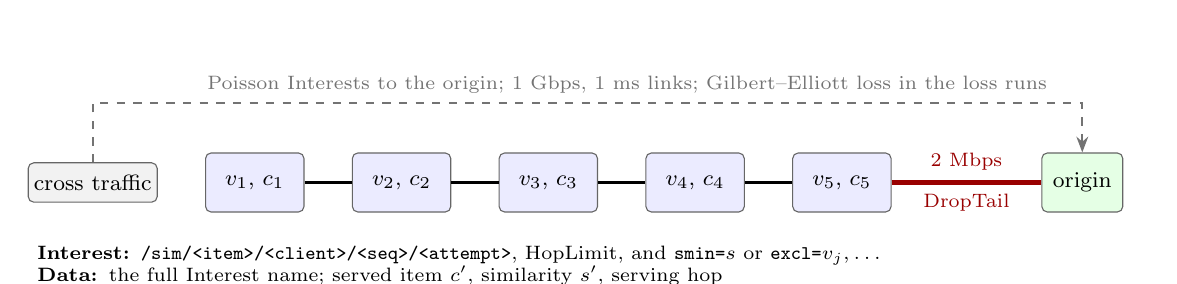
\begin{tikzpicture}[font=\footnotesize, node distance=0.6cm,
    cache/.style={bluebox, minimum width=1.25cm, minimum height=0.75cm}]
  \node[cache] (v1) {$v_1$, $c_1$};
  \foreach \i [count=\p] in {2,...,5} \node[cache, right=of v\p] (v\i) {$v_\i$, $c_\i$};
  \node[greenbox, minimum height=0.75cm, right=1.9cm of v5] (o) {origin};
  \foreach \a/\b in {v1/v2,v2/v3,v3/v4,v4/v5} \draw[thick] (\a) -- (\b);
  \draw[line width=2pt, red!60!black] (v5) -- node[above, font=\scriptsize] {2 Mbps}
        node[below, font=\scriptsize] {DropTail} (o);
  \node[graybox, minimum height=0.5cm, inner sep=2pt, left=0.6cm of v1] (x) {cross traffic};
  \draw[arr, dashed, black!55] (x.north) -- ++(0,0.75) -| node[pos=0.27, above, font=\scriptsize]
        {Poisson Interests to the origin; 1 Gbps, 1 ms links; Gilbert--Elliott loss in the loss
        runs} (o.north);
  \node[font=\scriptsize, align=left, anchor=north west, text width=14cm]
        at ([yshift=-0.3cm]x.south west |- v1.south)
        {\textbf{Interest:} \code{/sim/<item>/<client>/<seq>/<attempt>}, HopLimit, and
        \code{smin=}$s$ or \code{excl=}$v_j,\dots$\\
        \textbf{Data:} the full Interest name; served item $c'$, similarity $s'$, serving hop};
\end{tikzpicture}
\caption{System model: the base paper's tandem with a congested backhaul, cross traffic, burst loss
and our packet formats. Cache $v_i$ hosts client $c_i$, a similarity store and our strategy.}
\label{fig:system}
\end{figure}

\subsection{Answer-or-Forward Policies}\label{sec:policies}
When an Interest for item $c$ reaches cache $v$, the cache finds its closest stored item $c'$, with
similarity $s'$, and either replies with $c'$ or sends the Interest on. We compare four rules for
this choice.

\textbf{Blind (base paper).} The cache replies with probability $\alpha$ and forwards otherwise,
paying no attention to the user's threshold or to the delay upstream.

\textbf{Threshold.} The Interest carries the user's minimum similarity $s$, and the cache replies only
if $s'\geq s$ and its $\alpha$ coin also says yes. Every reply is then acceptable, so a request always
finishes in one attempt and Equation~(8) of the base paper holds exactly. Let $p_i$ be the
probability that the $i$-th cache on the path holds an acceptable item, $q_i=\alpha p_i$, $m$ the
number of caches before the origin and $\tau$ the delay of one link. The expected delay is then
\begin{equation}
\mathbb{E}[D_{\mathrm{thr}}] = \sum_{i=1}^{m} 2\tau(i-1)\,q_i\prod_{j<i}(1-q_j)
\;+\; 2\tau m\prod_{j=1}^{m}(1-q_j).
\label{eq:threshold-delay}
\end{equation}

\textbf{Exclusion.} Caches stay blind to the threshold, but after a rejection the client lists the
cache that answered in its next Interest. A listed cache forwards instead of repeating its answer, so
with $m$ caches on the path a request needs at most $m+1$ attempts.

\textbf{Delay-aware (ours).} Let $\Dup$ be the cache's estimate of the forwarding delay, $R_h$ the
round trip to a client $h$ hops away, and $F_v(s')$ the estimated share of $v$'s users who accept an
answer of similarity $s'$. Replying costs about $R_h$; if the client then rejects the answer, which
happens with probability $1-F_v(s')$, a further $\delta+R_h+\Dup$ is added. Forwarding costs
$R_h+\Dup$. The cache should therefore reply when
\begin{equation}
\bigl(1-F_v(s')\bigr)\bigl(\delta+R_h+\Dup\bigr)<\Dup
\iff
s'\geq s_v^*=F_v^{-1}\!\left(1-\frac{\Dup}{\delta+R_h+\Dup}\right).
\label{eq:decision-rule}
\end{equation}
The threshold $s_v^*$ moves with the measured upstream delay: the dearer forwarding becomes, the lower
the similarity a cache is willing to serve locally.

\subsection{Delay-Aware Algorithm}\label{sec:algo}
Algorithm~\ref{alg:delay-aware} keeps $\Dup$ as a smoothed round trip with gain $1/8$, as TCP does
for its timers~\cite{jacobson1988congestion,paxson2011rfc6298}; an expired Interest counts as the
time it wasted, so loss raises the estimate too. $F_v$ uses 20 similarity bins with a Laplace prior,
fitted to be non-decreasing. A retry that excludes $v$ marks $v$'s last answer as rejected, and no
retry within a window $W$ marks it as accepted. A verdict is uncertain while
Eq.~\eqref{eq:decision-rule} flips between $F_v\pm2$ standard errors; exploration stops once every
bin has settled.

\begin{algorithm}[H]
\caption{Delay-aware answer-or-forward decision at cache $v$}
\label{alg:delay-aware}
\begin{algorithmic}[1]
\Require Interest $I$ for item $c$ from a client $h$ hops away, exclusion list $E(I)$; store $B_v$;
         estimates $\Dup$, per-hop round trip $r$ and acceptance $F_v$
\State $c'\gets\arg\max_{x\in B_v}\operatorname{sim}(c,x)$; \quad $s'\gets\operatorname{sim}(c,c')$;
       \quad $R_h\gets hr$
\If{$v\in E(I)$}
  \State Record a rejection for the similarity previously served by $v$; forward $I$
\ElsIf{$s'=1$ \textbf{or} $(1-F_v(s'))(\delta+R_h+\Dup)<\Dup$ \textbf{or} the verdict is uncertain}
  \State Send Data$(\operatorname{name}(I);\, c',s',h)$ downstream; remember $(I,s',t_{\mathrm{now}})$
\Else
  \State Set $t_{\mathrm{fwd}}(I)\gets t_{\mathrm{now}}$ and forward $I$ upstream
\EndIf
\Statex \textit{On Data arrival or expiry for a forwarded Interest:}
\State $\Dup\gets\frac{7}{8}\Dup+\frac{1}{8}(t_{\mathrm{now}}-t_{\mathrm{fwd}}(I))$; update $r$
\Statex \textit{If no retry naming $v$ arrives within $W$ after an answer:}
\State Record an acceptance for similarity $s'$
\end{algorithmic}
\end{algorithm}

\subsection{Justification of the Design}\label{sec:justify}
\begin{itemize}
  \item \textbf{Bounding retries.} With blind caches and persistent contents, a user whose $m$
        nearby caches hold nothing acceptable gets through only if all $m$ forward, with probability
        $(1-\alpha)^m=10^{-5}$ at $\alpha=0.9$; in our runs the mean delay at $s=1$ jumps from the
        model's 80.6~ms to 14.5~s.
  \item \textbf{The role of $\alpha$.} Raising $q_i$ in Eq.~\eqref{eq:threshold-delay} moves
        probability from outcomes with delay at least $2\tau i$ to one with delay $2\tau(i-1)$, so
        under the threshold policy the delay falls as $\alpha$ grows and $\alpha=1$ is optimal.
  \item \textbf{Privacy and adaptation.} Neither exclusion nor the delay-aware rule needs the user's
        threshold, the delay-aware rule always serves an exact hit, and rising $\Dup$ lowers $s_v^*$.
  \item \textbf{Simulator constraints.} NFD matches exact names before our strategy runs, so the
        strategy does the similarity lookup and NFD stays unchanged. ndnSIM~2.9 bypasses ns-3's
        traffic control, so the bottleneck is a DropTail queue; we claim nothing about RED or CoDel.
\end{itemize}

% ================================================================ REFERENCES
\begin{thebibliography}{99}

\bibitem{zhang2014ndn}
L.~Zhang \emph{et al.}, ``Named data networking,'' \emph{ACM SIGCOMM Comput. Commun. Rev.},
vol.~44, no.~3, pp.~66--73, Jul. 2014,
doi: \href{https://doi.org/10.1145/2656877.2656887}{10.1145/2656877.2656887}.

\bibitem{neglia2022similarity}
G.~Neglia, M.~Garetto, and E.~Leonardi, ``Similarity caching: Theory and algorithms,''
\emph{IEEE/ACM Trans. Netw.}, vol.~30, no.~2, pp.~475--486, Apr. 2022,
doi: \href{https://doi.org/10.1109/TNET.2021.3126368}{10.1109/TNET.2021.3126368}.

\bibitem{schroeder2025vcache}
L.~G.~Schroeder \emph{et al.}, ``vCache: Verified semantic prompt caching,''
arXiv:2502.03771, 2025.

\bibitem{nakamura2024analysis}
R.~Nakamura and N.~Kamiyama, ``Analysis of similarity caching on general cache networks,''
\emph{IEEE Access}, vol.~12, pp.~163338--163348, 2024,
doi: \href{https://doi.org/10.1109/ACCESS.2024.3489620}{10.1109/ACCESS.2024.3489620}.

\bibitem{mastorakis2017ndnsim}
S.~Mastorakis, A.~Afanasyev, and L.~Zhang, ``On the evolution of ndnSIM: An open-source simulator
for NDN experimentation,'' \emph{ACM SIGCOMM Comput. Commun. Rev.}, vol.~47, no.~3, pp.~19--33,
2017, doi: \href{https://doi.org/10.1145/3138808.3138812}{10.1145/3138808.3138812}.

\bibitem{jacobson2009ccn}
V.~Jacobson, D.~K.~Smetters, J.~D.~Thornton, M.~F.~Plass, N.~H.~Briggs, and R.~L.~Braynard,
``Networking named content,'' in \emph{Proc. 5th Int. Conf. Emerging Networking Experiments and
Technologies (CoNEXT)}, 2009, pp.~1--12,
doi: \href{https://doi.org/10.1145/1658939.1658941}{10.1145/1658939.1658941}.

\bibitem{chaudhary2026ndncaching}
P.~Chaudhary, N.~Hubballi, and S.~G.~Kulkarni, ``Content caching methods in named data networks,''
arXiv:2605.13104, 2026.

\bibitem{falchi2008metric}
F.~Falchi, C.~Lucchese, S.~Orlando, R.~Perego, and F.~Rabitti, ``A metric cache for similarity
search,'' in \emph{Proc. ACM Workshop on Large-Scale Distributed Systems for Information Retrieval
(LSDS-IR)}, 2008, pp.~43--50,
doi: \href{https://doi.org/10.1145/1458469.1458473}{10.1145/1458469.1458473}.

\bibitem{pandey2009nn}
S.~Pandey, A.~Broder, F.~Chierichetti, V.~Josifovski, R.~Kumar, and S.~Vassilvitskii,
``Nearest-neighbor caching for content-match applications,'' in \emph{Proc. 18th Int. Conf. World
Wide Web (WWW)}, 2009, pp.~441--450,
doi: \href{https://doi.org/10.1145/1526709.1526769}{10.1145/1526709.1526769}.

\bibitem{bang2023gptcache}
F.~Bang, ``GPTCache: An open-source semantic cache for LLM applications enabling faster answers
and cost savings,'' in \emph{Proc. 3rd Workshop on NLP Open Source Software (NLP-OSS)}, 2023,
pp.~212--218, doi: \href{https://doi.org/10.18653/v1/2023.nlposs-1.24}{10.18653/v1/2023.nlposs-1.24}.

\bibitem{gill2025meancache}
W.~Gill, M.~Elidrisi, P.~Kalapatapu, A.~Ahmed, A.~Anwar, and M.~A.~Gulzar, ``MeanCache:
User-centric semantic caching for LLM web services,'' in \emph{Proc. IEEE Int. Parallel and
Distributed Processing Symp. (IPDPS)}, 2025, pp.~1298--1310,
doi: \href{https://doi.org/10.1109/IPDPS64566.2025.00117}{10.1109/IPDPS64566.2025.00117}.

\bibitem{gilbert1960capacity}
E.~N.~Gilbert, ``Capacity of a burst-noise channel,'' \emph{Bell Syst. Tech. J.}, vol.~39, no.~5,
pp.~1253--1265, Sep. 1960,
doi: \href{https://doi.org/10.1002/j.1538-7305.1960.tb03959.x}{10.1002/j.1538-7305.1960.tb03959.x}.

\bibitem{elliott1963estimates}
E.~O.~Elliott, ``Estimates of error rates for codes on burst-noise channels,'' \emph{Bell Syst.
Tech. J.}, vol.~42, no.~5, pp.~1977--1997, Sep. 1963,
doi: \href{https://doi.org/10.1002/j.1538-7305.1963.tb00955.x}{10.1002/j.1538-7305.1963.tb00955.x}.

\bibitem{jacobson1988congestion}
V.~Jacobson, ``Congestion avoidance and control,'' in \emph{Proc. ACM SIGCOMM}, 1988,
pp.~314--329, doi: \href{https://doi.org/10.1145/52324.52356}{10.1145/52324.52356}.

\bibitem{paxson2011rfc6298}
V.~Paxson, M.~Allman, J.~Chu, and M.~Sargent, ``Computing TCP's retransmission timer,'' IETF
RFC~6298, Jun. 2011.

\bibitem{sisalem2023acai}
T.~Si~Salem, G.~Neglia, and D.~Carra, ``Ascent similarity caching with approximate indexes,''
\emph{IEEE/ACM Trans. Netw.}, vol.~31, no.~3, pp.~1173--1186, Jun. 2023,
doi: \href{https://doi.org/10.1109/TNET.2022.3217012}{10.1109/TNET.2022.3217012}.

\bibitem{benmazziane2024ttl}
Y.~Ben~Mazziane, S.~Alouf, G.~Neglia, and D.~S.~Menasch\'{e}, ``TTL model for an LRU-based
similarity caching policy,'' \emph{Computer Networks}, vol.~241, Art. no.~110206, Mar. 2024,
doi: \href{https://doi.org/10.1016/j.comnet.2024.110206}{10.1016/j.comnet.2024.110206}.

\bibitem{garetto2021placement}
M.~Garetto, E.~Leonardi, and G.~Neglia, ``Content placement in networks of similarity caches,''
\emph{Computer Networks}, vol.~201, Art. no.~108570, Dec. 2021,
doi: \href{https://doi.org/10.1016/j.comnet.2021.108570}{10.1016/j.comnet.2021.108570}.

\bibitem{wang2025bandit}
L.~Wang \emph{et al.}, ``Similarity caching in dynamic cooperative edge networks: An adversarial
bandit approach,'' \emph{IEEE Trans. Mobile Comput.}, vol.~24, no.~4, pp.~2769--2782, Apr. 2025,
doi: \href{https://doi.org/10.1109/TMC.2024.3500132}{10.1109/TMC.2024.3500132}.

\end{thebibliography}

\end{document}
